\documentclass[aspectratio=169,10pt]{beamer}
\usepackage{booktabs}
\usepackage{graphicx}
\usepackage{tikz}
\usetikzlibrary{positioning,arrows.meta}
\graphicspath{{figures/dataset_slides/}{figures/data_quality/}}
\setbeamertemplate{navigation symbols}{}
\setbeamertemplate{footline}[frame number]
\newcommand{\mmh}{\,mm\,h$^{-1}$}

\title{Screening the OPERA archive for km-scale precipitation extremes}
\subtitle{Method, validation against gauges, and questions for MeteoSwiss}
\author{Filippo Quarenghi}
\institute{University of Lausanne}
\date{October 2026}

\begin{document}

\begin{frame}
  \titlepage
\end{frame}

% ===========================================================================
\section{Context}

\begin{frame}{Why the data matter for this project}
  \small
  \textbf{Task.} Super-resolution of precipitation from 25\,km to 2\,km over Europe
  ($128\times128$ tiles of 256\,km), deterministic and flow-matching models, with a structural
  loss built on Minkowski functionals of the rain field.
  \vspace{2mm}

  \textbf{Evaluation targets the tail}: exceedance ratios and return levels from a
  peaks-over-threshold fit at a fixed level (currently 31\mmh), and scores on 27 documented
  storms.
  \vspace{2mm}

  \textbf{So the data must provide:}
  \begin{itemize}
    \item a tail made of rain, not radar artefacts: these statistics rest on a few thousand
      pixels, and one undetected radar fault was 12\% of all test pixels above 89\mmh;
    \item splits that are independent in time, so test storms are not neighbours of training
      frames;
    \item test sets for shifts: documented extremes, and a change of radar product.
  \end{itemize}
\end{frame}

\begin{frame}{Data}
  \small
  \begin{itemize}
    \item EUMETNET OPERA rain-rate composite with quality index, open archive:
      \textbf{5,023 days, 2012-09 to 2026}, LAEA grid $2200\times1900$, 2\,km, 15\,min.
    \item \textbf{Two production chains}: ODYSSEY until 2024-07-05 (composite of the scans in
      a 15-min window), NIMBUS after (lowest-elevation scan at the nominal time). Earlier
      breaks: beam-blockage correction (2015), log $\to$ linear compositing (2017-09-29).
    \item \textbf{The raw field is dirty.} On a sample day (2018-06-15), 52 of 96 composites
      have a maximum above 500\mmh; the peak is 13,072\mmh.
    \item Independent truth for validation: 10-min gauges from DWD (1,454) and SwissMetNet
      (281), 12.1M station-frames.
  \end{itemize}
\end{frame}

% ===========================================================================
\section{Method}

\begin{frame}{Principles of the screen}
  \small
  \begin{enumerate}
    \item \textbf{Remove clear errors only; keep imperfections.} Blockage, attenuation,
      compositing seams and mild clutter stay, so the model learns to be robust to them.
    \item \textbf{Key every rule on an error signature}: geometry (rays, rings, range-only
      fields), persistence, exact repeated values, physical impossibility. Never on intensity
      or ``unusual structure'' alone, because real extremes are unusual too.
    \item \textbf{Repair pixels rather than drop tiles} where the artefact is local.
    \item \textbf{No labelled set.} Instead: rejection rate per intensity bin for every rule,
      the strongest flags of each rule looked at by eye, and validation against gauges.
    \item \textbf{The same screen for training and evaluation.}
    \item \textbf{The tail fit is an audit, never a rule.} Removing whatever makes the GPD fit
      better would select the data by the model used to evaluate it.
  \end{enumerate}
\end{frame}

\begin{frame}{Pipeline}
  \centering
  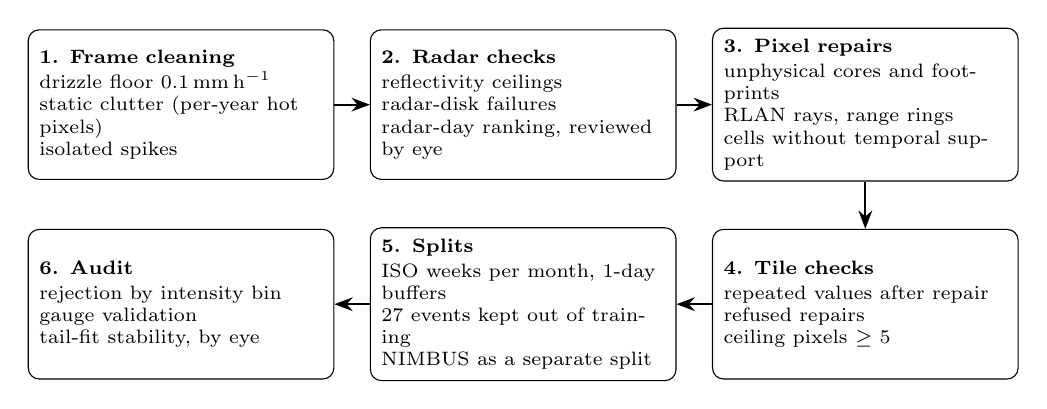
\begin{tikzpicture}[
      box/.style={draw, rounded corners, align=left, font=\scriptsize, text width=3.6cm,
                  minimum height=1.9cm, inner sep=4pt},
      arr/.style={-{Stealth}, thick}]
    \node[box] (a) {\textbf{1. Frame cleaning}\\[1pt]
      drizzle floor 0.1\mmh\\
      static clutter (per-year hot pixels)\\
      isolated spikes};
    \node[box, right=0.45cm of a] (b) {\textbf{2. Radar checks}\\[1pt]
      reflectivity ceilings\\
      radar-disk failures\\
      radar-day ranking, reviewed by eye};
    \node[box, right=0.45cm of b] (c) {\textbf{3. Pixel repairs}\\[1pt]
      unphysical cores and footprints\\
      RLAN rays, range rings\\
      cells without temporal support};
    \node[box, below=0.6cm of c] (d) {\textbf{4. Tile checks}\\[1pt]
      repeated values after repair\\
      refused repairs\\
      ceiling pixels $\ge$ 5};
    \node[box, left=0.45cm of d] (e) {\textbf{5. Splits}\\[1pt]
      ISO weeks per month, 1-day buffers\\
      27 events kept out of training\\
      NIMBUS as a separate split};
    \node[box, left=0.45cm of e] (f) {\textbf{6. Audit}\\[1pt]
      rejection by intensity bin\\
      gauge validation\\
      tail-fit stability, by eye};
    \draw[arr] (a) -- (b); \draw[arr] (b) -- (c); \draw[arr] (c) -- (d);
    \draw[arr] (d) -- (e); \draw[arr] (e) -- (f);
  \end{tikzpicture}
  \vspace{2mm}

  \raggedright\small
  Radar checks run on the field before any repair, so a repair cannot hide a failure. All
  decisions are stored as per-tile columns and applied at split time, so a threshold can
  change without reprocessing the archive.
\end{frame}

\begin{frame}{Frame cleaning and pixel repairs}
  \footnotesize
  \centering
  \renewcommand{\arraystretch}{1.3}
  \begin{tabular}{p{2.6cm}p{6.6cm}p{3.6cm}}
    \toprule
    rule & signature & action \\
    \midrule
    static clutter & pixel $\ge$ 31\mmh\ in $>$ 1\% of a calendar year's frames & neighbourhood median \\
    isolated spike & pixel $\ge$ 10\mmh, every neighbour $<$ 10\% of it & neighbour maximum \\
    unphysical core & pixel $>$ 500\mmh, with its connected region $\ge$ 150\mmh & median of the outer ring \\
    RLAN ray & thin component $\ge$ 80\,km aligned ($<$ 10°) with a radar within 250\,km & median of the outer ring \\
    range ring & circle in the per-year $\ge$ 31\mmh\ frequency around a site; pixels $\ge$ 89\mmh\ & median of the outer ring \\
    no temporal support & cell $\ge$ 10\mmh\ with no echo $\ge$ 1\mmh\ within 30\,km at $t\pm15$\,min & median of the outer ring \\
    \bottomrule
  \end{tabular}
  \vspace{3mm}

  \raggedright\small
  Nothing is zeroed. Tiles must be fully covered. The repair is guarded: a component above
  500 pixels is not repaired, and the tile is rejected instead.
\end{frame}

\begin{frame}{Failures that small, local or transient rules cannot see}
  \centering
  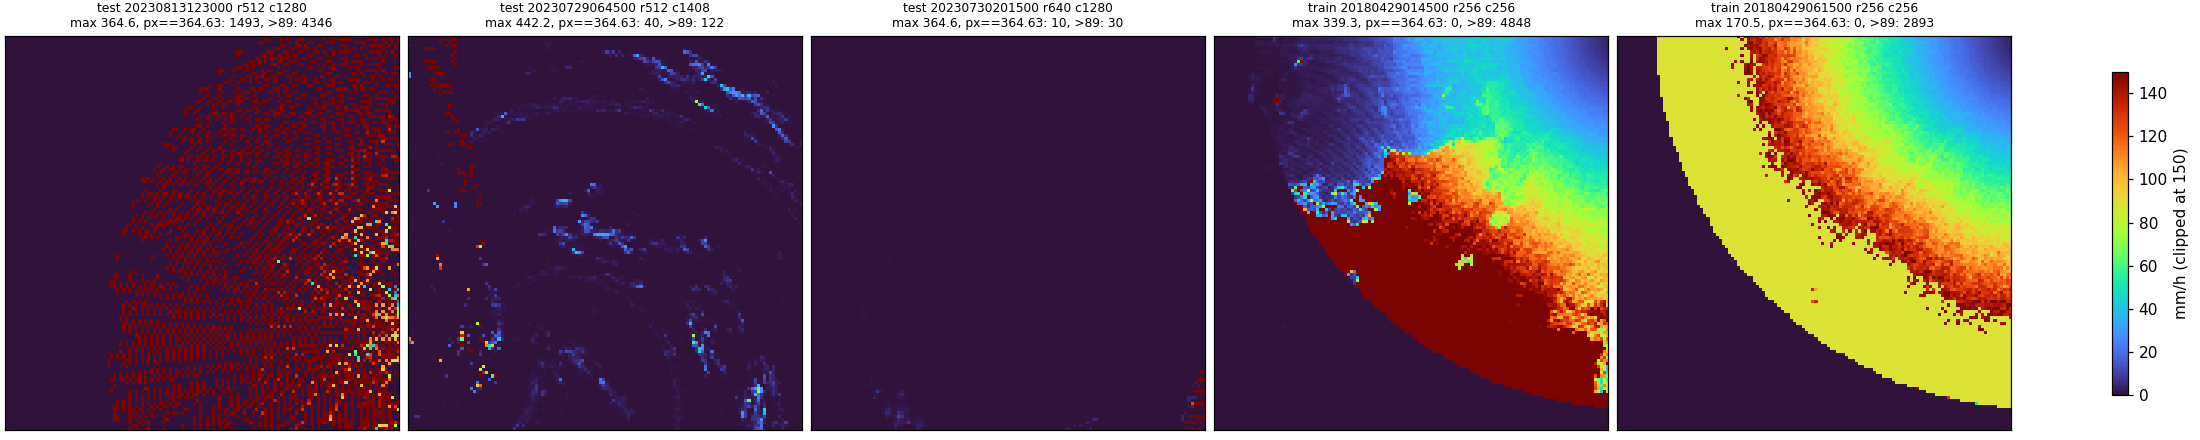
\includegraphics[width=\linewidth]{tail_suspects.png}
  \vspace{1mm}

  \raggedright\small
  \begin{itemize}
    \item \textbf{Reflectivity ceiling at 364.63\mmh\ = 64.0\,dBZ} ($Z = 200R^{1.6}$): speckle
      at one exact value inside real rain, Serbian and neighbouring radars, 2023.
    \item \textbf{Radar-disk failure}, Madrid (Torrejón), 2018-04-29: a smooth range-only field
      to 340\mmh\ over the whole disk; 16\% of all training pixels above 89\mmh.
    \item \textbf{Ceiling at 48.62\mmh\ = 50.0\,dBZ}, Oradea area, November 2019.
  \end{itemize}
  All three were found by the tail audit: $\xi(u)$ drifted instead of reaching a plateau.
\end{frame}

\begin{frame}{Radar-level checks}
  \small
  \textbf{Ceiling table} (per radar area and year). The count of a value is compared with the
  largest count of any other value within $\pm$4\,dB; a ceiling stands $\ge$ 5$\times$ above.
  Calibration: the known ceilings score 9.9--89, all other values have 99.9th percentile 1.96.
  Ceiling pixels are censored: $\ge$ 5 in a tile-frame reject it, 1--4 are repaired.
  \vspace{2mm}

  \textbf{Repeated value} (per tile, after repair). Real rain on the 0.01\mmh\ grid almost
  never repeats a value $\ge$ 31\mmh: per tail tile, median 1 repeat, 99.9th percentile 24.
  $\ge$ 50 rejects the tile; this also catches plateaus left by a repair.
  \vspace{2mm}

  \textbf{Radar-disk failure} (per radar and frame, over the area the radar owns): share of
  pixels $\ge$ 31\mmh, share of log-rate variance explained by range alone, and the jump in
  rate across the area boundary and the maximum-range circle. Real rain varies in azimuth.
  \vspace{2mm}

  \textbf{Radar-day ranking.} Each radar-day is scored against the radar's own seasonal
  99th percentile and the median of its 5 nearest radars on the same day:
  \[
    \text{score} = \log_{10}\frac{x + f}{\max(q_{99}^{\text{own}},\ \text{median}_{\text{neighbours}}) + f}
  \]
  on four signals: share $\ge$ 150\mmh, ceiling pixels, flagged frames, isolated high pixels.
  The top of the list is looked at; exclusions are decided by eye.
\end{frame}

\begin{frame}{Splits}
  \small
  \begin{itemize}
    \item \textbf{Blocked in time}: whole ISO weeks drawn per calendar month, 1-day buffers;
      every test day is at least 2 days from any training day.
    \item \textbf{Documented extremes}: 27 storms from published case studies (MeteoSwiss,
      DWD, ESSL, AEMET, Météo-France, ECMWF), with their whole week, kept out of training
      (25 in test, 2 in the NIMBUS split); every tile kept.
    \item \textbf{Product shift}: train, validation and test are ODYSSEY only; NIMBUS days are
      a separate test split.
    \item Stratified sampling by tile maximum with inclusion weights, so the tail is
      oversampled and statistics can be reweighted.
  \end{itemize}
  \vspace{2mm}
  \centering
  \begin{tabular}{lrrrr}
    \toprule
    & train & validation & test & NIMBUS \\
    \midrule
    patches & 1,962,057 & 252,809 & 297,460 & 487,673 \\
    event tiles & -- & -- & 36,166 (25 events) & 5,249 (2 events) \\
    \bottomrule
  \end{tabular}
  \vspace{1mm}

  \raggedright\footnotesize Sizes of the current build (before the radar-level checks).
\end{frame}

% ===========================================================================
\section{Validation}

\begin{frame}{Validation against gauges: design}
  \small
  \begin{itemize}
    \item 1,735 DWD and SwissMetNet 10-min gauges, 12.1M station-frames on 4,968 days. The radar
      frame matches the gauge interval 10--20\,min later (log-rate correlation 0.29--0.47).
    \item Gauge quality control on the gauges alone: fault codes, stuck runs, isolated bursts
      with no rain at any gauge within 30\,km.
    \item \textbf{Presence}: does the gauge see rain ($\ge$ 1\mmh) under a pixel? Per rule and
      intensity bin.
    \item \textbf{Values}: exceedance ratio over the same station-frames, with no conditioning
      on either side:
      \[ \rho(u) = \frac{N(\text{radar} \ge u)}{N(\text{gauge} \ge u)} \]
      A flat $\rho$ means the radar has the gauges' tail \emph{shape}. Its level mixes
      point-vs-area and instantaneous-vs-10-min differences, which are not quantified.
  \end{itemize}
\end{frame}

\begin{frame}{Presence: the rules remove artefacts, tile rejection removes rain}
  \footnotesize
  \centering
  Share of pixels with gauge $\ge$ 1\mmh, by radar intensity:
  \vspace{1mm}

  \begin{tabular}{lccccc}
    \toprule
    class & [10,31) & [31,89) & [89,150) & [150,500) & $\ge$500 \\
    \midrule
    untouched & 0.91 & 0.92 & 0.91 & 0.90 & -- \\
    no temporal support & 0.01 & 0.01 & 0.00 & 0.00 & 0.01 \\
    range ring & 0.82 & 0.50 & 0.00 & 0.00 & 0.00 \\
    spike repaired & 0.13 & 0.24 & 0.24 & 0.26 & 0.00 \\
    other pixels of tiles rejected as unphysical & 0.81 & 0.74 & 0.55 & 0.10 & 0.05 \\
    \bottomrule
  \end{tabular}
  \vspace{2mm}

  \raggedright\small
  \begin{itemize}
    \item Temporal support is the cleanest rule. Rings carry real rain below 31\mmh\ and none
      from 89\mmh, hence ring repair only from 89\mmh.
    \item A tile rejected for one bad pixel is usually a real storm: repair the pixel instead.
    \item Repaired pixels: the gauge saw $\ge$ 10\mmh\ under 5.3\% of them (untouched: 44.6\%).
    \item The quality index does not separate real from false tail pixels.
  \end{itemize}
\end{frame}

\begin{frame}{Values: is the tail calibrated?}
  \begin{columns}[T]
    \begin{column}{0.52\textwidth}
      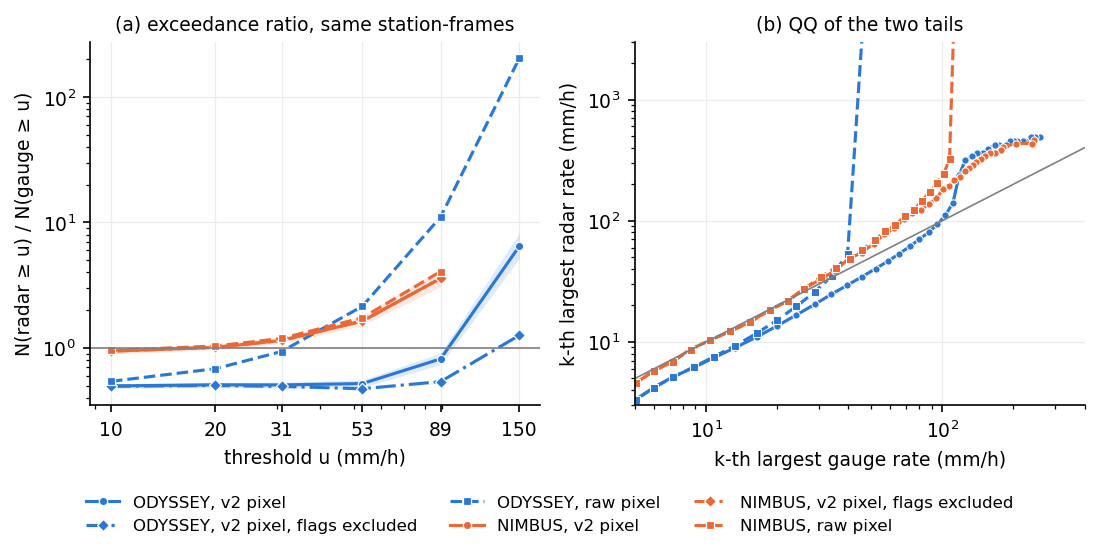
\includegraphics[width=\linewidth]{fig_gauge_values.png}
    \end{column}
    \begin{column}{0.46\textwidth}
      \footnotesize
      \begin{tabular}{lccc}
        \toprule
        $\rho(u)$ & 31 & 89 & 150 \\
        \midrule
        ODYSSEY raw & 0.93 & 11.0 & 204 \\
        ODYSSEY, cleaned & 0.51 & 0.82 & 6.5 \\
        \quad + flags excluded & 0.49 & 0.54 & 1.26 \\
        \quad + pixel repairs & -- & 0.57 & 1.47 \\
        NIMBUS, cleaned & 1.14 & 3.6 & 31 \\
        \bottomrule
      \end{tabular}
      \vspace{2mm}

      \footnotesize
      \begin{itemize}
        \item \textbf{ODYSSEY}: the radar exceeds u about half as often as the gauges, at
          every level up to 89\mmh\ once flagged pixels are excluded. The tail shape matches; an
          excess of 2.5--3$\times$ remains at 150\mmh\ ($\approx$100 gauge exceedances).
        \item \textbf{NIMBUS}: heavier than the gauges from $\approx$31\mmh. The pixels are rain
          (96\% have rain at the gauge at 150--500\mmh), and no rule touches them.
        \item At gauge $\ge$ 30\mmh, median radar/gauge ratio 0.45.
      \end{itemize}
    \end{column}
  \end{columns}
\end{frame}

\begin{frame}{ODYSSEY and NIMBUS on the same days}
  \small
  101 days held in both products (2,407 frames, 97,682 wet tiles):
  \vspace{2mm}

  \centering
  \begin{tabular}{lc}
    \toprule
    quantity & NIMBUS / ODYSSEY \\
    \midrule
    wet area $\ge$ 0.1 / 1\mmh & 0.71 / 0.99 \\
    exceedance $\ge$ 10 / 31 / 89\mmh & 1.36 / 1.44 / 2.4 \\
    perimeter of the 10--31\mmh\ excursion sets & $\approx$1.8 \\
    spectral power at 128 / 32 / 8 / 4\,km & 1.25 / 1.42 / 3.1 / 6.2 \\
    +15\,min frame correlation & 0.41 $\to$ 0.26 \\
    \bottomrule
  \end{tabular}
  \vspace{2mm}

  \raggedright
  NIMBUS fields are more intense, rougher and more fragmented at small scales, consistent with
  an instantaneous scan against a 15-min composite. A model trained on ODYSSEY pays a product
  penalty on NIMBUS that is unrelated to extremeness, so NIMBUS is scored against
  same-product references only.
\end{frame}

% ===========================================================================
\section{Status}

\begin{frame}{When is the dataset ready? A gate fixed in advance}
  \small
  The dataset is ready when one more cleaning step would not change any reported number.
  \begin{enumerate}
    \item \textbf{Known failures absent}, from a regression catalogue.
    \item \textbf{Residual contamination measured}: 100 random test tiles with max $\ge$ 89\mmh\
      looked at; 95\% upper bound on the artefact rate $\le$ 5\%.
    \item \textbf{Stable reference}: dropping the 20 most influential non-event days moves no
      observed tail statistic outside its day-block bootstrap interval.
    \item \textbf{Real extremes survive}: $<$ 0.5\% of tiles rejected per event; no rule's
      rejection rate rises steeply with intensity; gauge $\rho$ no worse than before.
    \item \textbf{Remaining drift in $\xi(u)$ explained} by a named cause (truncation,
      regional mixing, sub-asymptotic threshold).
  \end{enumerate}
  \vspace{2mm}
  \textbf{Calibration so far} (199 days: known failures, 27 events, 100 random days): every
  known failure caught (the remaining tiles of those days checked by eye); worst event 0.14\%
  of tiles rejected; random-day rejection $\le$ 0.014\% below 150\mmh. The full-archive radar
  pass is running.
\end{frame}

\begin{frame}{Open issues}
  \small
  \begin{itemize}
    \item \textbf{Isolated high clusters.} Clusters of 2--9 pixels at 40--340\mmh\ in dry
      surroundings survive on the Oradea days. A per-tile rule would also remove 9--16\% of
      event tiles, so they are handled per radar-day, against the radar's neighbours.
    \item \textbf{486.2\mmh\ = 66.0\,dBZ} is the maximum of 55 tiles; no nearby value is the
      maximum of more than 3. A product-level cap would make the tail censored there.
    \item \textbf{11.53\mmh\ = 40.0\,dBZ} piles up on three of the radars that carry the 64\,dBZ
      ceiling in 2023.
    \item \textbf{NIMBUS tail excess} over the gauges, untouched by any rule.
    \item \textbf{Quality index inverted under ODYSSEY}: unconfirmed tail pixels have the
      higher index (median 0.90 vs 0.20).
    \item \textbf{Validation covers Germany and Switzerland only}; the failures above were in
      Serbia, Spain and Romania.
  \end{itemize}
\end{frame}

% ===========================================================================
\section{Questions for MeteoSwiss}

\begin{frame}{Questions: artefacts and screening}
  \small
  \begin{enumerate}
    \item Which artefact types does MeteoSwiss see in the OPERA composite that this screen
      misses? Which composite-level filters do you trust (texture, satellite cloud masks,
      others), and with which thresholds?
    \item Are \textbf{reflectivity ceilings} at round dBZ values (64.0, 50.0, 40.0, and
      possibly 66.0\,dBZ) known for OPERA, and is 66\,dBZ a cap applied by the compositing?
    \item How do you tell a \textbf{small intense core} from a \textbf{cluster of clutter
      pixels} without volume data? Is a radar-day comparison with neighbouring radars a
      sensible test?
    \item \textbf{Repair or reject?} For ML training sets, do you repair artefact pixels or
      drop the sample? Any experience of models learning repaired values?
    \item Why would the OPERA \textbf{quality index} be higher on unconfirmed tail pixels under
      ODYSSEY, and carry no signal under NIMBUS? Is it usable in any form?
  \end{enumerate}
\end{frame}

\begin{frame}{Questions: tail calibration and plausibility}
  \small
  \begin{enumerate}
    \setcounter{enumi}{5}
    \item Is a factor $\approx$0.5 between ODYSSEY and gauge exceedance counts expected, from
      Z--R and from comparing a 2\,km pixel with a point?
    \item \textbf{NIMBUS rates heavy rain above the gauges}, increasingly with intensity
      (1.15$\times$ the gauge exceedances at 31\mmh, 3.6$\times$ at 89\mmh). Is this known?
      Instantaneous scan vs 10-min totals, hail, or the NIMBUS processing? This decides
      whether NIMBUS can serve as a test set.
    \item What is a defensible \textbf{upper plausibility bound} for a 15-min, 2\,km rate? We
      use 500\mmh, with repair down to 150\mmh\ around such cores.
    \item Should a \textbf{hail cap} (e.g.\ above $\approx$55\,dBZ) be applied before any tail
      statistic?
    \item How should the \textbf{product breaks} (2015, 2017, 2024) be handled when pooling
      years for training?
  \end{enumerate}
\end{frame}

\begin{frame}{Questions: defining and measuring extremes}
  \small
  \begin{enumerate}
    \setcounter{enumi}{10}
    \item How does MeteoSwiss define intense precipitation for \textbf{radar rates} at 2\,km
      and 5--15\,min, as opposed to accumulation-based warning levels? Is a fixed 31\mmh\
      meaningful, or should the level be regional, seasonal or product-specific?
    \item \textbf{Rate or accumulation?} Should the tail be defined on 1-h accumulations,
      which are impact-relevant and comparable with gauges? 15-min snapshots miss short peaks
      (Valencia 2024: 28.6\mmh\ at the radar pixel vs a 184.6\mmh\ gauge-hour).
    \item \textbf{Peaks over threshold from radar}: how do you choose the threshold, decluster
      exceedances in space and time, and choose between pixel-level and event-maximum fits?
      How do you report return levels from radar?
  \end{enumerate}
\end{frame}

\begin{frame}{Questions: independent truth and out-of-distribution tests}
  \small
  \begin{enumerate}
    \setcounter{enumi}{13}
    \item Can we access \textbf{CombiPrecip and POH/MESHS for 2012--2026}? The open portal
      keeps 14 days.
    \item Which \textbf{shift} matters operationally for downscaling: unprecedented
      intensities, Alpine orography, new radars or products, future climate, or NWP input
      (ICON-CH1/2)?
    \item Would \textbf{Switzerland held out} be a meaningful test, with CombiPrecip and the
      gauges as independent truth? Is a held-out region meaningful when every country has its
      own network?
    \item Above which rate does the radar tail stop being trustworthy as a test target for
      an \textbf{intensity cut-off} experiment? In mm/h or relative to local climate?
    \item Is there an \textbf{event catalogue} (TRT tracks, hail, lightning) that could label
      storm types across the archive? How does MeteoSwiss evaluate its own ML nowcasting on
      unseen extremes?
    \item Would MeteoSwiss \textbf{validate the Swiss part} of a released benchmark, or
      co-own it?
  \end{enumerate}
\end{frame}

\begin{frame}{The three answers that unblock the most}
  \small
  \begin{enumerate}
    \item \textbf{The plausibility bound and the 66\,dBZ question} (Q2, Q8, Q9): they decide
      whether the tail above $\approx$490\mmh\ is truncated, censored or capped, and how the
      tail fit is done.
    \item \textbf{The NIMBUS excess} (Q7): it decides whether the NIMBUS split is a product
      robustness test or a biased reference.
    \item \textbf{CombiPrecip and POH/MESHS access} (Q14): an independent truth over
      complex terrain, for validating the screen and for an out-of-distribution test.
  \end{enumerate}
\end{frame}

\end{document}
